\section{\review{Observables}}

% ============================================
%               Dispersion
% ============================================
\subsection{\review{Dispersion}}

Treating a beam as a single particle having the design momentum $p_0$ leads to a machine with no
apparent ill effect related to that momentum.
However, when considering a particle beam where each particle follows a distribution in
momentum, a few effects arise from this deviation, called the \textit{momentum offset},
$\delta$. It is defined as a relative difference to the design momentum:

\begin{equation}
    \delta = \frac{p - p_0}{p_0}.
    \label{eq:coordinate_systems:momentum_offset}
\end{equation}

Those effects are referred to as \textit{chromatic aberrations}. The first and most important to
consider is the \textit{dispersion}. Dispersion results from a particle with a momentum offset
being deflected differently by the dipoles compared to a particle at the design momentum.
\Cref{fig:coordinate_systems:dispersion} shows an example of deflection. 
The particle is still subject to the other properties of the lattice, but with a different orbit,
described by the dispersion function in \cref{eq:coordinate_systems:dispersion}.

\begin{figure}[!htb]
    \centering
    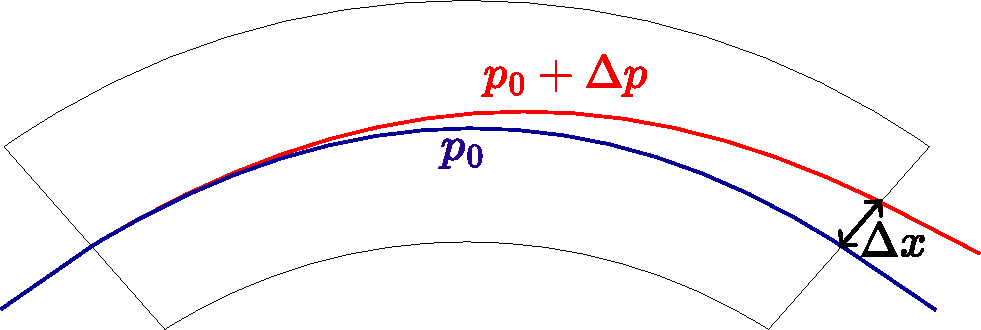
\includegraphics[width=0.6\textwidth]{images/dipole.pdf}
    \caption{Particles with a momentum offset will be deflected differently by dipoles. This offset
            in position can be described by the dispersion function.}
    \label{fig:coordinate_systems:dispersion}
\end{figure}

\begin{equation}
    \begin{aligned}
    D_x(s) = \frac{\Delta x(s)}{\delta} \\
    D_y(s) = \frac{\Delta y(s)}{\delta}.
    \end{aligned}
    \label{eq:coordinate_systems:dispersion}
\end{equation}

\FloatBarrier

% --------------------------------------------
%         Momentum Compaction Factor
% --------------------------------------------
\paragraph{\review{Momentum Compaction Factor}}
\label{subsection:coordinates_systems:momentum_compaction_factor}

In synchrotrons, particles with a deviation in momentum with respect to the reference particle will
experience a different path length due to the bending of the dipoles. This effect is characterized
by the \textit{momentum compaction factor}~\cite{wiedemann_particle_2015},

\begin{equation}
    \alpha_c = \frac{\Delta C / C}{\delta},
\end{equation}

relating the circumference of the ring $C$ to the momentum offset $\delta$.
A positive momentum compaction factor indicates a longer path traveled by particles with a positive
momentum offset, and vice versa.


The momentum compaction factor can also be broken down into orders as an infinite sum, where the
constant term is often referred to as the first order,

\begin{equation}
    \alpha_c = \underbrace{\alpha_{c,0}}_{\text{Constant term}}
               + \underbrace{\sum_{i \geq 1} \alpha_{c, i} \delta^i}_\text{Linear and non linear terms}.
\end{equation}

In the LHC, the contribution from the non constant terms is
negligible~\cite{keintzel_jacqueline_beam_2022}. Further details can be found
in~\cref{subsection:decapoles:chromaticity:measurement}.

\FloatBarrier

% ============================================
%               Beta Function
% ============================================
\subsection{\review{$\beta$-function}}

As seen previously in~\cref{section:courant_snyder}, the $\beta$-function is related to the amplitude
of oscillations of the beam. \Cref{fig:beam_optics:beta} shows how the $\beta$-function
oscillates along the ring due to quadrupoles focusing and defocusing properties.
The $\beta$-function is an important quantity found as a factor in several other observables that
will be described later in this thesis.


\begin{figure}[H]
    \centering
    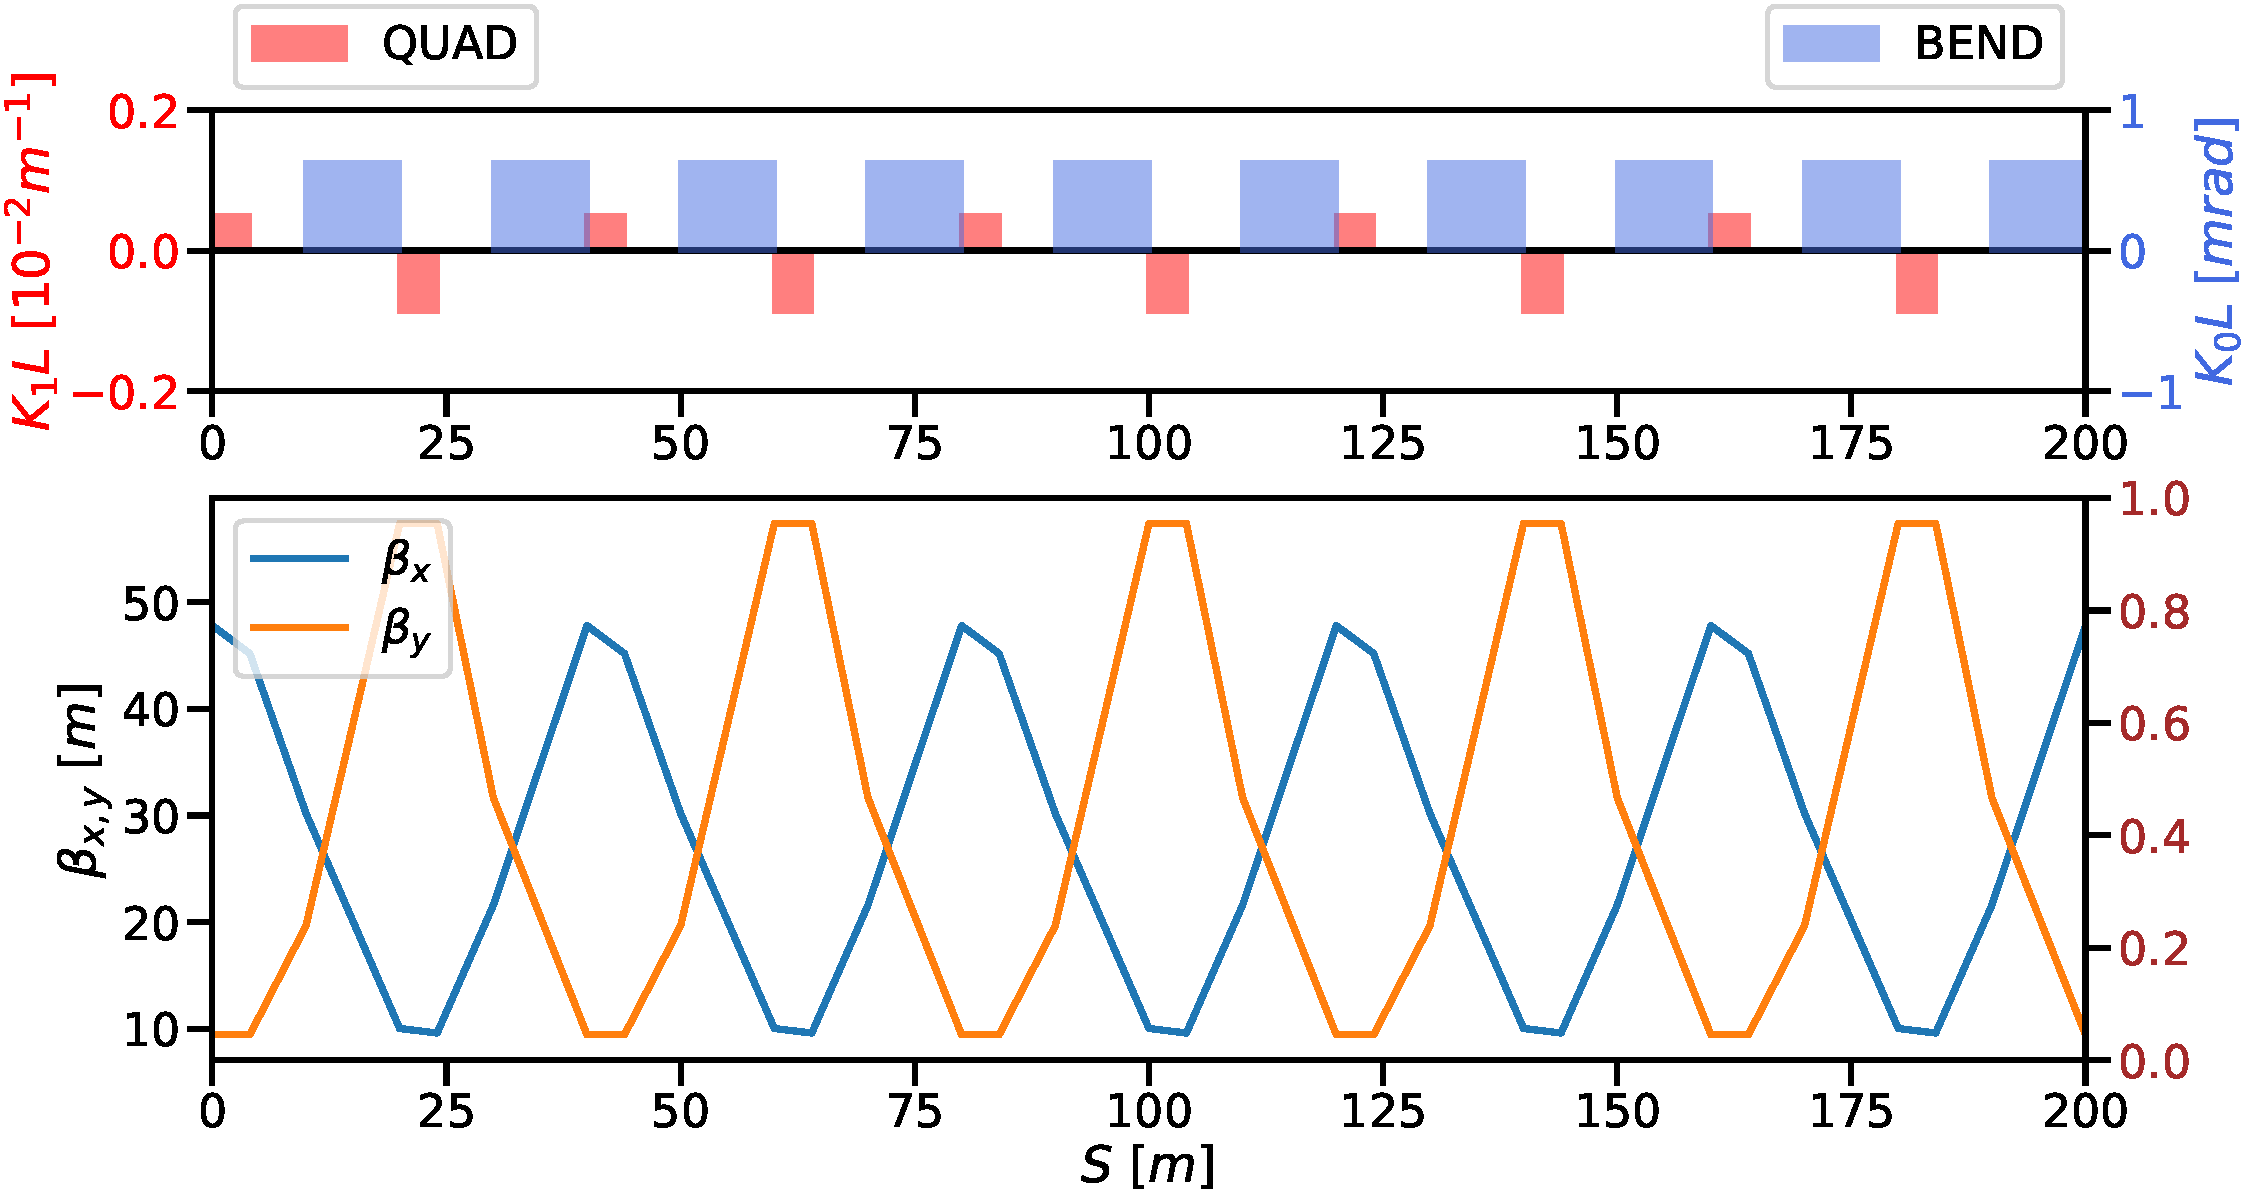
\includegraphics[width=0.9\textwidth]{images/beta_function.pdf}
    \caption{Evolution of the $\beta$-function along the lattice. Horizontal and vertical beatings
    are usually opposite given the focusing and defocusing properties of quadrupoles in each plane.}
    \label{fig:beam_optics:beta}
\end{figure}

A difference in $\beta$-function compared to the design leads to possibly unstable and larger beams,
degrading its properties and making it harder to control. The relative difference in
$\beta$-function is called the beta-beating, expressed in percents: 

\begin{equation}
    \beta-\mathrm{beating \; [\%]}  = \frac{\beta_z(s) - \beta_z(s)_{model}}{\beta_z(s)_{model}}.
    \label{eq:beam_optics:beating}
\end{equation}


% ============================================
%                  Coupling
% ============================================
\subsection{\review{Coupling}}

In a perfect scenario, the particle motion of each transverse plane is independent, or
\textit{uncoupled}. In practice, this transverse motion can be altered by some magnetic elements,
giving rise to \textit{betatron coupling} where the motion of each plane is not independent anymore.
Such elements can be quadrupoles, mounted with a roll error introducing skew-quadrupolar fields,
which are the main source of linear coupling in the LHC~\cite{felix_soubelet_local_2023}. Field
imperfections, solenoids and feed-down from higher orders can also contribute to coupling.

The resonances $Q_x + Q_y$ and $Q_x - Q_y$, called the \textit{sum} and \textit{difference}
resonances, are mainly excited by skew quadrupoles. When coupling is present in the
machine, the former may lead to unstable motion while the latter introduces an periodic exchange of
emittance between the planes, keeping it stable. They can be characterized by the RDTs $f_{1010}$
and $f_{1001}$.

Effects of normal multipoles start showing their skew counterpart (and vice versa) as the motion
of transverse planes become coupled. This is demonstrated in \cref{chapter:skew_octupole_fields}
with octupoles.

